\documentclass[letterpaper, 11pt]{article} 

\usepackage{graphics,graphicx}
\usepackage{multicol} 
\usepackage{parskip}
\usepackage{amsmath}
\usepackage{multirow}
\usepackage[utf8]{inputenc}
\usepackage{fancyhdr}
\usepackage[title]{appendix}
\usepackage{wasysym}
\usepackage{url}
\usepackage{subcaption}

\usepackage[font=footnotesize,labelfont=small]{caption}
\captionsetup{width=0.85\linewidth}

\RequirePackage{geometry}
\geometry{margin=2cm}

\setlength{\parskip}{0.2cm}
\setlength{\parindent}{0pt}


\title{Project 2 Report: Bank-level Parallelism and Memory Controller Design}
\author{
Tai Duc Nguyen \\
ECEC 623: Advanced Topics in Computer Architecture
}
\date{\today}

\begin{document}

\maketitle


%----------------------------------------------------------------------------------------
%	ABSTRACT
%----------------------------------------------------------------------------------------

\rule{\textwidth}{1pt}

\begin{abstract}
	In modern von-Neuman computing systems, the processing unit is often limited by the amount of information allowed to flow between it and the memory. Hence, in order to maximize this bandwidth resource, memory controller designs, like FR-FCFS, are created. While this legacy design works well for a single application situation, it can massively slow down programs in a system where multiple programs are executed in parallel by allowing a few memory hungry applications to dominate the bandwidth. For this reason, many researchers have introduced a lot of complexity to the design of FRFCFS to attack this problem of "unfair memory scheduling". Nonetheless, the paper \textit{"BLISS: Balancing Performance, Fairness and Complexity in Memory Access Scheduling"} by Subramanian et. al demonstrated that the BLISS design can be fair while requiring minimal amount of complexity. The authors showed that BLISS achieves 25\% better fairness than the best-performing memory scheduler for benchmarks from the SPEC CPU2006 suite, TPC-C, Matlab and the NAS parallel benchmark suite. However, this project will put BLISS to the test when fared against various heavy machine learning workloads. The results from this experiment only show that BLISS has a 1.7\% (on average) fairness improvement when compared to FR-FCFS.
\end{abstract}

\rule{\textwidth}{1pt}

\section{Experimental Setup}

In our experimental setup, we use an approximated algorithm for FRFCFS whose only goal is to maximize the memory bandwidth. On every clock cycle, our FRFCFS implementation fills as many memory instructions into the banks as much as possible. The "fairness" of this greedy algorithm is compared against the modified BLISS algorithm, whose prioritizations are as follow (1 as the most important criteria):

\begin{enumerate}
	\item Non-blacklisted application’s requests
	\item Requests hit to a free bank (FRFCFS)
	\item Older requests.
\end{enumerate}

The blacklisted status are calculated as follow:

\begin{enumerate}
	\item If the last application ID is the same as the one being served, increase the counter for that application ID by 1
	\item If such counter exceed the \textit{blacklisting threshold}, mark that application ID as \textbf{blacklisted}
	\item If the last application ID is different than the one being served, reset the counter for the last application ID to 0
	\item The blacklisting status will be reset after N cycles.
\end{enumerate}

In our setup, the \textit{blacklisting threshold} is set to be 4 and the blacklisting reset is N = 10000 cycles.

Same as project 1, some assumptions used in the experiment are:
\begin{enumerate}
	\item DRAM Memory timings are:
	\begin{enumerate}
		\item Reading takes 53 clock cycles
		\item Writing takes 53 clock cycles
	\end{enumerate}
	\item PCM Memory timings are:
	\begin{enumerate}
		\item Reading takes 57 clock cycles
		\item Writing takes 162 clock cycles
	\end{enumerate}
	\item Maximum number of requests in the waiting queue is: 64
	\item The number of banks being tested are: 8, 16
	\item FR-FCFS loop searching for new request when the first one has bank-conflict can be done in 1 clock cycle
\end{enumerate}

The memory traces used are generated using a Hybrid-eDRAM-PCM computer simulator running different machine learning workloads. Their names and short-handed symbols are:

\begin{enumerate}
	\item CNN (C)
	\item Bi-directional RNN (BR)
	\item Variational Autoencoder (VAE)
	\item Autoencoder (AE)
	\item Nearest neighbor (NN)
	\item Word2vec (W2V)
	\item RNN (R)
	\item Random Forest (RF)
	\item Kmeans (K)
	\item Linear Regression (LIR)
	\item DCgan (DCG)
	\item GAN (G)
	\item Logistic Regression (LOR)
	\item Dynamic RNN (DR)
	\item Neural Network (NRN)
\end{enumerate}

From these ML application workloads, 5 traces are created where each consists of a unique combination of 8 different ML workloads above:

\begin{enumerate}
	\item Trace 1: C-BR-VAE-AE-NN-W2V-R-RF
	\item Trace 2: C-VAE-NRN-NN-BR-RF-W2V-R
	\item Trace 3: K-LIR-DCG-BR-W2V-NRN-AE-LOR
	\item Trace 4: NN-K-NRN-W2V-C-AE-LIR-VAE
	\item Trace 5: R-AE-NN-W2V-DR-C-G-VAE
\end{enumerate}

\section{Results and Discussion}

This section details the results from the simulation with graphs.

\begin{figure}[htb!]
	\centering
	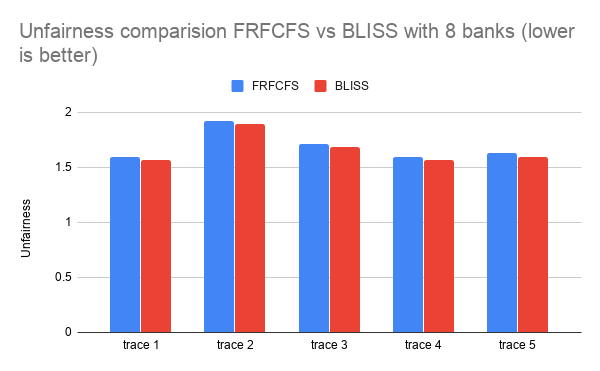
\includegraphics[width=0.7\linewidth]{unfair_8banks.png}
	\caption{Unfairness metrics comparision between BLISS and FRFCFS on 5 ML traces and 8 banks}
	\label{fig1}
\end{figure}

\begin{figure}[htb!]
	\centering
	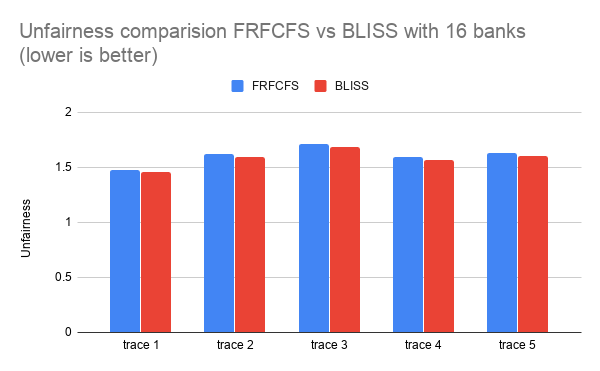
\includegraphics[width=0.7\linewidth]{unfair_16banks.png}
	\caption{Unfairness metrics comparision between BLISS and FRFCFS on 5 ML traces and 16 banks}
	\label{fig2}
\end{figure}

\begin{figure}[htb!]
	\centering
	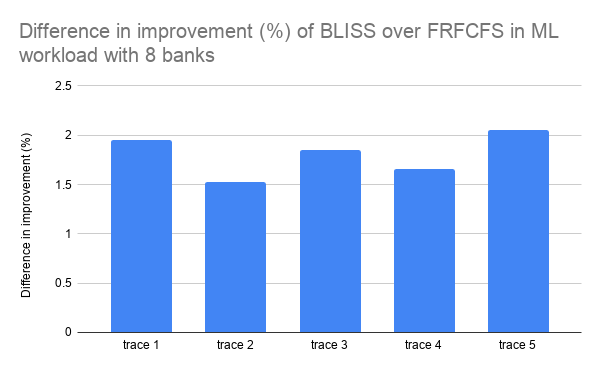
\includegraphics[width=0.7\linewidth]{improvement_8banks.png}
	\caption{Improvement of BLISS over FRFCFS (in \%) with 8 banks}
	\label{fig3}
\end{figure}

\begin{figure}[htb!]
	\centering
	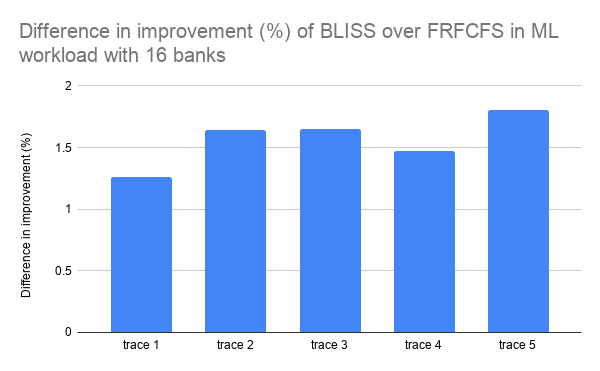
\includegraphics[width=0.7\linewidth]{improvement_16banks.png}
	\caption{Improvement of BLISS over FRFCFS (in \%) with 16 banks}
	\label{fig4}
\end{figure}

\newpage

From these results, it is apparent that BLISS is a more \textit{fair} memory scheduler than FRFCFS; however, not by much. This low improvement (compare to the paper by Subramanian et. al) is likely due to the fact that the number of applications running simultaneously (on 8 banks) is 16, 24, and 32, which can induces a lot more interference. In addition, the effect of the modification of FRFCFS and BLISS algorithms is unknown and hard to predict. 

\end{document}